\section{Privacy and Data Protection in Emerging Scenario}
Negli ultimi anni abbiamo assistito ad una continua crescita di:
\begin{itemize}
    \item database di governi e aziende
    \item contenuti generati e caricati da utenti, messi a disposizione di fruitori attraverso piattaforme come YouTube, Flickr..
    \item informazioni identificative di persone, raccolte ogni qual volta una persona si registra ad un sito, effettua la login ad un'applicazione, si registra a una newsletter, partecipa a un sondaggio..
\end{itemize}
E si sono sempre più diffusi:
\begin{itemize}
    \item metodi e motivi di distribuzione di dati 
    \begin{itemize}
        \item per effettuare degli studi sui trend o per eseguire inferenze statistiche
        \item condividere conoscienze
        \item accedere a servizi online
    \end{itemize}
    \item storage e dispositivi di calcolo esterni, con i vantaggi di:
    \begin{itemize}
        \item diminuire i costi a dispetto dei servizi offerti
        \item grande disponibilità dei servizi e protezione da disservizi di ogni genere 
    \end{itemize}
\end{itemize}
Questo ci porta a voler/dover garantire la privacy e l'intergrità dei dati.

\subsection{Privacy in Data Publication}
Come abbiamo già detto in precedenza, il problema della privatezza nasce quando ho dei dati e voglio condividerli. Solitamente, in passato, i dati venivano usati per scopi statistici e potevamo avere:
\begin{itemize}
    \item DBMS statistici dove l'utente interroga il DBMS con query statistiche, il DMBS interroga il DB e restituisce la statistica all'utente. Quest'ultimo non può chiedere un dato specifico, ma solo un'aggregazione dei dati (somma, media...)
    \item Dati statistici dove chi ha il DB produce le statistiche e poi le pubblica.
\end{itemize}
Possiamo da subito renderci conto che le policy per garantire la sicurezza dei dati devono essere diverse tra questi due sistemi, infatti:
\begin{itemize}
    \item nel primo caso il controllo deve essere dinamico perchè è l'utente che esegue la query a runtime. Le cose principali da controllare sono:
    \begin{itemize}
        \item range della query: se il target è troppo piccolo rischio di esporre un singolo individuo, se è troppo grande rischio di esporre piccoli gruppi (perchè posso fare un'intersezione tra gruppo e gruppo più grande per avere come risultato il gruppo più piccolo).
        \item storico delle query: window history
        \item collusione: quando due o più parti si mettono insieme per fare query che da soli non avrebbero potuto fare
    \end{itemize}
    \item nel secondo caso invece è l'owner del db che decide cosa pubblicare, quindi effettua un controllo di tipo statico
\end{itemize}
\subsubsection{Macrodati vs Microdati}
Possiamo definire dei dati come macrodati quando rilascio statistiche e quando rispondo a query statistiche ossia quando non pubblico i dati veri e propri. I macrodati possono essere identificati in due gruppi (tipi di tabelle):
\begin{itemize}
    \item tabelle di conteggio/frequenza dove ogni cella contiene il numero di rispondenti o della percentuale di rispondenti
    \begin{center}
        \begin{figure}[h!]
          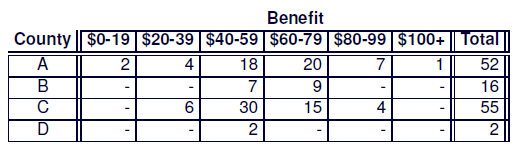
\includegraphics[scale=0.8]{img/counttable.png}
          \caption{Tabella bidimensionale che mostra il conteggio dei beneficiari diviso per dimensione del benefit e contea}
        \end{figure}
    \end{center}
    \item tabelle di grandezza dove ogni cella della tabella contiene un valore aggregato di una determinata quantità di interesse.
    \begin{center}
        \begin{figure}[h!]
          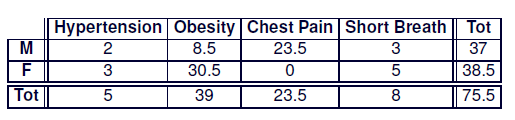
\includegraphics[scale=0.8]{img/magtable.png}
          \caption{Media del numero di giorni passati in ospedale dato un disturbo}
        \end{figure}
    \end{center}
\end{itemize}
Quando pubblichiamo dei dati dobbiamo sempre stare attenti a proteggere la privacy di chi sta dietro i dati. Ma esattamente cosa significa proteggere la privacy?
\begin{itemize}
    \item proteggere l'identità (identity disclosure: un rispondente è identificato dai dati rilasciati)
    \item proteggere l'informazione sensibile (attribute disclosure: informazioni sensibili riguardanti un rispondente emergono dal rilascio dei dati). Devo stare attento sia quando pubblico dati precisi (es. un numero esatto) sia quando posso fare inferenza (es. valore in un range da 1.3 a 1.7: essendo un range piccolo posso esporre un singolo individuo)
    \item bloccare la possibilità di fare inferenza sui dati (inferential disclosure: i dati rilasciati rendono possibile la determinazione di caratteristiche riguardanti un rispondente anche se non sono mai stati rilasciati dati su di lui) dove non è la singola informazione ad essere sensibile, ma la possobilità di fare inferenza su di essa la rende sensibile. Ad esempio: il data mining ha lo scopo di trovare correlazioni tra dati, tramite le correlazioni posso fare inferenze e quindi arrivare a dati sensibili.
\end{itemize}

Nel caso in cui ci sia la identity disclosure un utente terzo è in grado di identificare un rispondente dai dati rilasciati. 
Abbiamo però una differenza tra macrodati e microdati:
\begin{itemize}
    \item macrodati: rivelare l'identità non è generalmente un problema fino a quando l'identificazione porta a divulgare informazioni confidenziali (attribute disclosure)
    \item microdati: l'identificazione è un serio problema siccome i microdati sono dettagliati e l'identity disclosure implica anche l'attribute disclosure
\end{itemize}

L'inferential disclosure avviene quando le informazioni possono essere ricavate da proprietà statistiche dei dati rilasciati. 
Questa non sempre rappresenta un rischio:
\begin{itemize}
    \item dati statistici vengo rilasciati apposta per permettere agli utenti di fare inferenze e capire le relazioni tra le variabili
    \item le inferenze sono progettate per prevedere comportamenti aggregati, non di individui singoli e sono anche metodi poco precisi per predire dati di singoli
\end{itemize}

Un primo passo per evitare tutte queste disclosure è sicuramente quello di restringere i dati e restringere l'accesso ai dati: devo limitare i dati che pubblico nelle tabelle (restricted data) e nello stesso tempo devo avere un accesso ristretto, ossia imporre condizioni di accesso ai dati (restricted access). Ad esempio i dati li posso dare solo a certe identità e per certi specifici scopi (purpose of use). \\
I microdati includono intrinsecamente identificatori espliciti (nome, indirizzo ip, email) e devono essere tolti perchè sono sensibili e identificanti.\\
Ulteriori restrizioni potrebbero essere: l'inserimento di un timing entro il quale i dati possono essere tenuti e il divieto di divulgazione ad altri.\\

\subsubsection{Protezione per conteggio e frequenza dei macrodati}
Questo tipo di dati include il conteggio di valori o le percentuali di risposte ad un determinato sondaggio.\\
Per proteggere questi tipi di dati abbiamo diverse tecniche:
\begin{itemize}
    \item campionamento: pubblicare un sondaggio al posto che un censimento
    \item regole speciali: specificare delle restrizioni sul livello di dettaglio dei dait
    \item regole soglia: definisce una determinata cella di una tabella come sensibile se il numero dei rispondenti è minore di un numero specificato
\end{itemize}

\subsubsection{Tecniche di protezione per microdati}
Le più usate tecniche di protezione dei microdati possono essere classificate come segue:
\begin{itemize}
    \item masking techniques: trasformo il set originale di dati non rilasciandoli o perturbandoli
    \begin{itemize}
        \item non perturbative: i dati originali non vengono modificati ma alcuni dati vengono soppressi e altri rimossi (sampling local suppression, generalization)
        \item perturbative: i dati originali vengono modificati aggiungendo del rumore (rounding,swapping)
    \end{itemize}
    \item synthetic data generation techniques: rilascio dati plausibili sintetici, ma non quelli originali
    \begin{itemize}
        \item fully synthetic: il set dei dati rilasciati contiene solo dati sintetici
        \item partially synthetic: il set dei dati rilasciati contiene un mix di dati originali e sintetici
    \end{itemize}
\end{itemize}

\subsubsection{Il problema dell'anonimità}
I dati vengono de-identificati prima di essere rilasciati, ossia vengono rimossi tutti quei dati indentificanti (nome, cognome ...), ma questo non è sufficiente. Questi dati possono essere usati per unire identità con informazioni de-identificate per eseguire un processo di re-identificazione.

\subsubsection{Classificazione degli attributi nelle tabelle di microdati}
\begin{itemize}
    \item identificatori: identificano univocamente un rispondente (codice fiscale)
    \item quasi-identificatori: attributi che messi in combinazione con altri possono permettere la reidentificazione
    \item confidenziali: attributi che contengono informazioni sensibili (malattia di un paziente)
    \item non confidenziali: attributi che non sono da considerarsi sensibili e il quale rilascio non causa nessun problema di divulgazione
\end{itemize}

\subsubsection{Fattori che contribuiscono a rischi nella divulgazione}
Sempre parlando di microdati questi fattori possono genereare rischi nella divulgazione:
\begin{itemize}
    \item esistenza di high visiblity records: alcuni record che possono rappresentare caratteristiche uniche come lavori insoliti o stipendi alti
    \item possibilità di matchare microdata con altre informazioni esterne: esistono individui nella popolazione che possiedono combinazioni di caratteristiche univoche e se queste vengono prese come campione posso generare un disclosure risk.
\end{itemize}
Oppure posso generare la possibilità di unire dati o aumentare la loro precisione con:
\begin{itemize}
    \item tanti attributi comuni tra tabelle di microdati e sorgenti esterne
    \item accuratezza e precisione dei dati (es. data nascita completa o anno di nascita)
    \item numero e ricchezza delle fonti esterne
\end{itemize}

\subsubsection{Fattori che contribuiscono alla diminuzione dei rischi nella divulgazione}
\begin{itemize}
    \item le tabelle di microdati solitamente contengono un subset della popolazione, quindi può essere che l'utente malevolo non trovi quello che sta cercando
    \item molte volte i dati recenti non sono disponibili, ma sono accessibili solo quelli più vecchi che creano così un disallineamento temporale
    \item nelle tabelle di microdati c'è sempre un po'di rumore, dovuto anche a errori
    \item i dati vengono espressi in formati diversi e quindi è più difficile fare la correlazione
\end{itemize}

\subsubsection{Misure di rischio}
Per misurare il rischio nella divulgazione dobbiamo considerare:
\begin{itemize}
    \item la probabilità che il rispondente di cui l'intruso sta cercando informazioni abbia delle informazioni sia nei microdati che in file esterni
    \item la probabilità che gli stessi valori presenti nei microdati e nei file esterni siano stati salvati in un modo che siano collegabili
    \item la probabilità che il rispondente cui l'intruso sta cercando informazioni sia unico nella popolazione presente nel file esterno
\end{itemize}
Se un individuo è unico nella popolazione, allora sarà unico anche in ogni subset. Se invece un individuo è unico in un subset, non per forza sarà unico anche nella popolazione.

\subsection{K-anonymity}
Garantire privacy in senso assoluto non è un'operazione così facile. Di solito ci si limita a garantire un certo livello di anonimità. Per questo entra in gioco k-anonimity che insieme a generalizzazione e soppressione è stato proposto come approccio per proteggere l'identità del rispondente.\\
K-anonimity ha lo scopo di garantire che i dati rilasciati non possono essere ricollegati a un numero minore di k persone.\\ L'idea che sta alla base è quella di non poter utilizzare i quasi identificatori per eseguire operazioni di linking. \\
Ogni release di dati sarà fatta in modo che ogni combinazione di valori di quasi identificatori può essere collegata ad almeno k rispondenti. Quindi k-anonymity richiede che ogni valore quasi identificatore che appare nella tabella deve avere almeno k occorrenze (condizione sufficiente).\\
Ogni rilascio di dati quindi avrà almeno k persone che sembrano uguali.
\subsubsection{Generalizzazione e soppressione}
\begin{itemize}
    \item generalizzazione: il valore di un attributo è sostituito utilizzando valori più generici basato sulla definizione di una generalizzazione gerarchica (al posto che pubblicare tutta la data di nascita, pubblico solo l'anno)
    \item soppressione: tolgo il dato sensibile (così facendo potrei ridurre il numero di generalizzazioni necessarie a soddisfare il vincolo di k-anonymity)
\end{itemize}

\subsubsection{DGH - Domain Generalization Hierarchy}
L'idea è quella di costruire per ogni dominio una gerarchia di generalizzazioni che mi dice come andare da un valore più specifico ad uno più generico.
Definiamo \(\leq_D\) come una relazione di generalizzazione che definisce un mapping tra il dominio D e le sue generalizzazioni.\\
Dati due domini \(D_i\) e \(D_j\) \in Dom, \(D_i \leq_D D_j\) vuol dire che i valori nel dominio \(D_j\) sono generalizzazioni dei valori in \(D_i\). \\
\(\leq_D\) implica l'esistenza, per ogni dominio D, di una \(DGH_D = (Dom, \leq_D)\):
\begin{itemize}
    \item \(\forall D_i, D_j, D_z\in Dom:\) \\
    \(D_i \leq_D D_j\), \(D_i \leq_D D_z\) \Longrightarrow  \(D_j \leq_D D_z \lor D_z \leq_D D_j\)\\
    questa condizione significa ordine totale (catena). I domini sono in relazione a catena.
    \item L'elemento massimale (la radice della catena) è singleton (ossia ha dentro un solo valore).
\end{itemize}
L'ordine totale a livello di domini è una catena mentre a livello di tuple di domini è un reticolo (lattice) poichè è il cartesiano delle catene:\\
\( DT = <D_1,...,D_n> | D_i\) \in Dom \(\forall i=1,...,n \) la DGH di DT è: 
\(DGH_{DT} = DGH_{D1} x ... x DGH_{Dn}\)\\\\
\clearpage
Per esempio una generalizzazione di un singolo attributo (dominio) potrebbe essere:
\begin{center}
    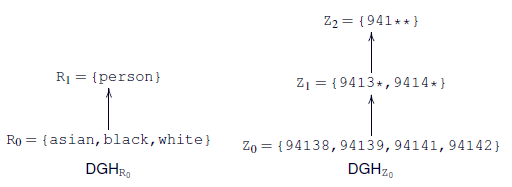
\includegraphics[scale=0.7]{img/chaingener.png}
\end{center}
Dove \(R_1\) e \(Z_2\) sono singleton.\\
Mentre la generalizzazione di una tupla di domini potrebbe essere:
\begin{center}
    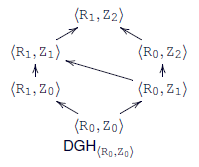
\includegraphics[scale=0.7]{img/retgen.png}
\end{center}
Come possiamo notare dalla foto abbiamo un reticolo il che comporta le seguenti proprietà:
\begin{itemize}
    \item ho una relazione d'ordine
    '\item ho un elemento top e uno bottom
    \item ho transitività e antisimmetria ossia se una cosa sta sotto a un'altra e l'altra sta sotto di lei, allora stiamo parlando della stessa cosa
\end{itemize}

\subsubsection{VGH - Value Generalization Hierarchy}
Definiamo \(\leq_V\) come una relazione di valori di generalizzazione che associa ad ogni valore in un dominio \(D_i\) un valore unico nel dominio \(D_j\), generalizzazione diretta di \(D_i\).\\
\(\leq_V\) implica l'esistenza, per ogni dominio D, di un valore gerarchico di generalizzazione \(VGH_D\), rappresentato da un albero dove:
\begin{itemize}
    \item le foglie sono i valori in D
    \item la radice (ossia il valore più generico) è il valore dell'elemento massimo in \(DGH_D\)
\end{itemize}
Il fatto che sia un albero ci permette di poter dire con certezza che ogni elemento ha un solo padre, cioè c'è un solo cammino che porta un elemento alla radice.
\begin{center}
    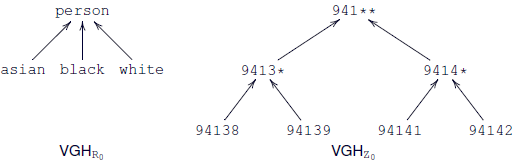
\includegraphics[scale=0.7]{img/vgh.png}
\end{center}
\subsubsection{Tabelle generalizzate tramite la soppressione}
Siano \(T_i\) e \(T_j\) due tabelle definite dagli stessi attributi. La tabella \(T_j\) è la generalizzazione (tramite soppressione delle tuple) della tabella \(T_i\). Questo viene denotato come \(T_i \preceq T_j\) se:
\begin{enumerate}
    \item \(|T_j| \leq |T_i|\) ossia ha un numero minore o uguale di tuple (a livello di cardinalità) 
    \item il domino \(dom(A, T_j)\) di ogni attributo A in \(T_j\) è uguale a, o è una generalizzazione di, il dominio \(dom(A, T_i)\) di ogni attributo A in \(T_i\), ossia per ogni valore in \(T_j\) è una generalizzazione dello stesso valore in \(T_i\)
    \item è possibile definire una funzione iniettiva che associa ogni tupla \(t_j\) in \(T_j\) tale per cui il valore di ogni attributo in\(t_j\) è uguale a, o è una generalizzazione di, il valore del corrispondente attributo in \(t_i\). Tale funzione non può essere biettiva perchè alcune tuple specifiche non "vanno" alla tabella generale perchè non sono state fatte soppressioni
\end{enumerate}
La generalizzazione deve essere eseguita nei giusti termini perchè se è troppo poca rischio di esporre i dati, mentre se è troppa i dati rischiano di non avere più senso.
\begin{center}
    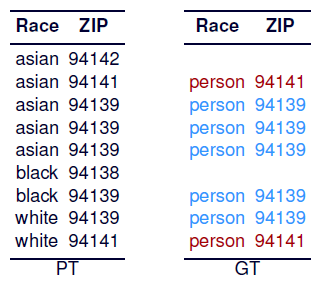
\includegraphics[scale=0.7]{img/tabgen.png}
\end{center}
La tabella riportata sopra ha k-anonymity uguale a 2 poichè il gruppo più piccolo è composto da 2 persone (evidenziate in rosso). 
Le tuple nella tabella GT inoltre non sono associate a tutte quelle della tabella PT (visto che abbiamo soppresso e generalizzato). Possiamo notare anche come la funzione non sia biettiva (biunivoca) infatti non possiamo risalire alla tabella specifica avendo quella generalizzata.
\subsubsection{Generalizzazione k-minimale con soppresione}
Definiamo il Distance vector usando come esempio il reticolo visto in precedenza.\\
Siano \(T_i(A_1,...,A_n)\) e \(T_j(A_1,...,A_n\) due tabelle tali che \(T_i \preceq T_j\). Il distance vector da \(T_j\) a \(T_i\) è il vettore \(DV_{ij}=[d_1,...d_n]\), dove ogni \(d_z\) con z = 1,...,n è la lunghezza del cammino unico tra \(dom(A_z, T_i)\) e \(dom(A_z,T_j)\) nel dominio di generalizzazione gerarchica \(DGH_D_z\)
\begin{center}
    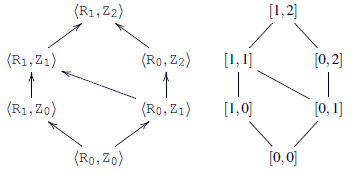
\includegraphics[scale=0.7]{img/dv.png}
\end{center}
Per calcolare la lunghezza del distance vector devo fare la somma, ad esempio: per andare da [0,0] a [1,2] ho tre salti poichè ho generalizzato 1 volta R e 2 volte Z.\\\\
Siano \(T_i(A_1,...,A_n)\) e \(T_j(A_1,...,A_n\) due tabelle tali che \(T_i \preceq T_j\) e sia MaxSup la soglia specifica di soppressione accettata. \(T_j\) è una generalizzazione k-minimale di \(T_i\) se:
\begin{enumerate}
    \item \(T_j\) soddisfa la k-anonymity facendo la minima soppressione richiesta (minimal suppression): \(T_j\) deve cancellare solo le tuple che servono per soddisfare k-anonymity, cioè non ci sono altre tabelle con la stessa k-anonymity cancellando meno tuple.
    \item \(|T_i| - |T_j| \leq MaxSup \) ossia non sopprimo più di quanto richiesto
    \item \(\forall T_z: T_i \preceq T_z\) e \(T_z\) soddisfa le condizioni 1 e 2 \Longrightarrow \(\lnot (DV_{i,z} < DV_{i,j}) \) cioè non ci deve essere un vettore più specifico che fa la stesso lavoro. 
\end{enumerate}
Per esempio, prendendo il DV della figura riportata in precedenza (ed escludendo ai fini dell'esempio [0,0] e [0,1]), se [1,0] mi basta allora [1,1] e [1,2] non vanno bene. [0,2] invece è okay perchè sta generalizzando su altro.
\begin{center}
    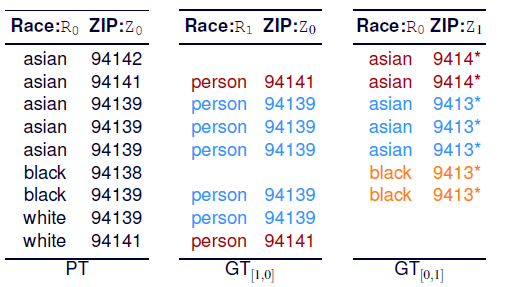
\includegraphics[scale=0.7]{img/maxsup.png}
\end{center}
In questo esempio abbiamo usato MaxSup = 2 e come possiamo vedere dalla foto sia la seconda che la terza tabella hanno dv uguale a uno rispetto alla prima tabella.

\subsubsection{Criteri soggettivi e oggettivi di scelta}
Possono essere applicati diversi criteri oggettivi di preferenza per scegliere tra due generalizzazioni minimali, come per esempio:
\begin{itemize}
    \item \textbf{minimum absolute distance}: si preferisce la generalizzazione con la distanza assoluta minore, cioè con il numero minore di passi di generalizzazione effettuati. Questo ovviamente non è una soluzione ottimale in alcuni casi, infatti non tiene conto della differenza dei domini: nel nostro caso se generalizziamo la colonna Race le persone diventano tutte uguali, se generalizzo con Zip no
    \item\textbf{ minimum relative distance}: non considero ciascun passo con un valore 1, ma lo peso rispetto a dove si colloca nella gerarchia, prendendo quindi quello che relativamente generalizza di meno. Ad esempio: [1,0] fa 1 passo di generalizzazione su una gerarchia alta 1 (cioè \(\frac{1}{1} + \frac{0}{1} = 1 \)) mentre [0,1] fa un passo su una gerarchia alta 2 (cioè \(\frac{0}{1} + \frac{1}{2} = \frac{1}{2}\)). Scegliamo quindi il secondo.
    \item \textbf{maximum distribution}: si preferisce la generalizzazione con il più grande numero di tuple distinte, cioè che lascia una certa diversità tra gruppi di tuple che rispettano comunque la k-anonymity scelta. Nel nostro caso la seconda soluzione dato che crea 3 gruppi invece di due (evidenziati in arancio, azzurro e rosso)
    \item \textbf{minimum suppression}: si preferisce la generalizzazione che sopprime meno tuple, cioè la generalizzazione è quella che mantiene la cardinalità più alta. Nel nostro caso non potremmo adottare questo criterio poichè entrambe le istanze eliminano 2 tuple 
\end{itemize}
Per quanto riguarda i criteri soggettivi invece dobbiamo valutarli noi in base al contesto.
\subsubsection{Granularità di generalizzazione e soppressione}
Entrambi questi metodi possono essere applicati a diversi livelli di granularità:
\begin{itemize}
    \item la generalizzazione può essere applicata a livello di singola colonna (applico a tutta la colonna la generalizzazione) o singola cella (diverse celle della stessa colonna possono avere diversi livelli di generalizzazione)
    \item la soppressione può lavorare a livello di riga (rimuovo la tupla), colonna (oscuro i valori di una colonna) e singola cella (una tabella k-anonima può essere ottenuta rimuovendo solo determinate celle)
\end{itemize}
Il tutto può essere riassunto tramite la seguente tabella:
\begin{center}
    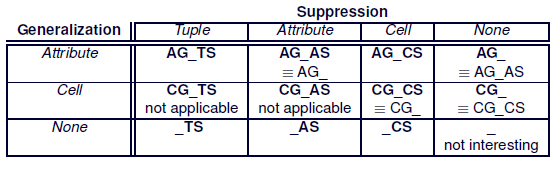
\includegraphics[scale=0.7]{img/granularity.png}
\end{center}
dove AG\_TS significa AttributeGeneralization\_TupleSuppression.\\
Non applicabile significa che non applico le soluzioni che fanno generalizzazione a granularità fine, ma soppressione a granularità più spessa.
\subsubsection{Esempi di tabelle 2-anonymized}
\begin{center}
    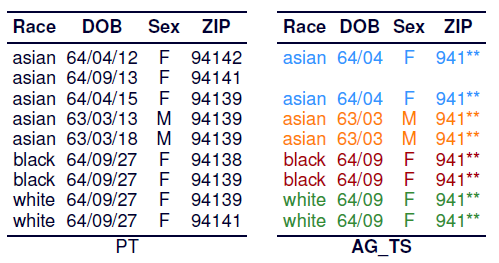
\includegraphics[scale=0.6]{img/2anon1.png}
\end{center}
La prima soluzione potrebbe essere quella di cancellare l'intera tupla e generalizzare lo ZIP in modo che l'ultima colonna abbia valori uguali
\begin{center}
    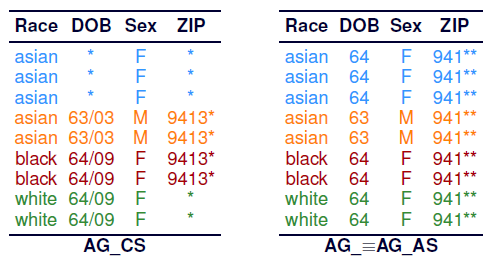
\includegraphics[scale=0.6]{img/2anon2.png}
\end{center}
La seconda soluzione nasce dalla generalizzazione della data di nascita e dello ZIP, sopprimendo solo alcuni di questi valori a livello di cella.\\
La terza soluzione si limita a generalizzare la data di nascita e lo ZIP.
\begin{center}
    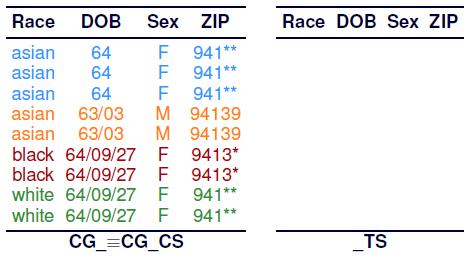
\includegraphics[scale=0.6]{img/2anon3.png}
\end{center}
La quarta soluzione nasce dall'aver effettuato generalizzazioni di diverso livello sulle celle delle colonne DOB e ZIP.\\
La quinta soluzione potrebbe essere una tuple suppression di tutte le tuple
\begin{center}
    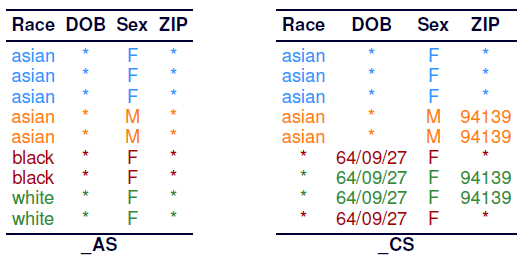
\includegraphics[scale=0.6]{img/2anon4.png}
\end{center}
La sesta soluzione nasce dalla soppressione completa delle colonne DOB e ZIP.\\
La settima e ultima soluzione proposta nasce dalla soppressione di celle in quasi tutte le colonne.\\\\
Operare a granularità più fine ha come vantaggio l'avere una maggiore utilità in quanto posso lasciare più informazioni nella tabella, ma ha come svantaggi il fatto che:
\begin{enumerate}
    \item ho una relazione eterogenea: i domini dell'attributo sono eterogenei, cioè diversi, e quindi ho problemi di query
    \item il costo computazionale della tabella cresce di molto
\end{enumerate}

\subsubsection{Algoritmi per calcolare una tabella k-anonima}
Il problema di trovare una tabella k-anonima minimale con generalizzazione di attributi e soppressione delle tuple (AG\_TS) è computazionalmente difficile (NP-HARD): ciò che rende il problema complicato è quindi la ricerca della soluzione minimale, cioè sopprimere e generalizzare solo quel che serve, escludendo tutte le altre soluzioni che "ci sono sopra".
La k-anonimity è stata pensata alla fine degli anni ‘90 ma la complessità computazionale è troppo alta (la maggioranza degli algoritmi “esatti” proposti hanno un tempo computazionale esponenziale rispetto al numero degli attributi che compongono i quasi identificatori). Quindi questi algoritmi sono pratici quando il numero QIdegli attributi nell’insieme dei quasi-identificatori è piccolo comparato al numero delle tuple n nella tabella privata PT.
Negli anni sono stati proposti numerosi algoritmi per produrre tabelle che rispettino k-anonimity attraverso la generalizzazione e la soppressione di tuple (cioè tramite AG\_TS). Questo perché con AG\_TS possiamo lavorare a livello di schema, perché tengo il problema della ricerca k-minimale nella sua formulazione più semplice.\\\\

\subsection{Algoritmi per AG\_TS e AG}
Partiamo con un esempio: so che [0,0] non soddisfa, [1,2] soddisfa. Che calcoli devo fare?\\ Posso provare tutti i cammini, sia dall’alto che dal basso, e vedere quale combinazione soddisfa.Guardando la gerarchia \(DGH_{DT}\) vediamo che ogni soluzione ha un cammino che posso prendere partendo dalla tabella base oppure dalla tabella più generale. Se la soluzione corrente non soddisfa i requisiti cambio soluzione, spostandomi in profondità o in ampiezza. Ma in questo modo sto percorrendo tutti i cammini che è computazionalmente oneroso. \\\\

Ogni cammino \(DGH_{DT}\) rappresenta una strategia di generalizzazione della tabella PT.\\
Chiamo \textbf{generalizzazione minima locale} il nodo più basso per ogni cammino che soddisfa k-anonimity.\\
Questo algoritmo porta con se due proprietà:
\begin{enumerate}
    \item ogni generalizzazione che è minimale globalmente è anche minimale localmente
    \item più salgo nella gerarchia, meno tuple devo rimuovere per garantire k-anonymity
\end{enumerate}
Ne deriva che se non hai una soluzione che garantisce k-anonymity e che sopprime meno di MaxSup tuple all’altezza h, allora non puoi avere soluzioni ad altezza più bassa di h (dove per altezza si intende la distanza dalla “radice”).\\\\
L'algoritmo utilizza una ricerca dicotomica (ricerca binaria) sul reticolo DV:
\begin{enumerate}
    \item valuta la soluzione ad altezza h/2
    \item se esiste una soluzione che soddisfa k-anonymity
    \begin{itemize}
        \item valuta la soluzione ad altezza h/4
        \item altrimenti valuta la soluzione a 3h/4
    \end{itemize}
    \item fino a che l'algoritmo raggiunge l'altezza minima per la quale c'è un DV che soddisfa k-anonymity
\end{enumerate}
Per ridurre i costi computazionali viene adottata una \textbf{matrice distance vector} per evitare la computazione di ogni tabella generalizzata
\begin{center}
    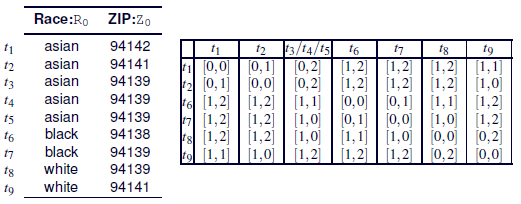
\includegraphics[scale=0.6]{img/dvmatrix.png}
\end{center}
Analizziamo la tabella:
\begin{itemize}
    \item ognuno è distante [0,0] da sè stesso
    \item t1 e t2 diventano uguali con [0,1] cioè con un passo di generalizzazione sullo ZIP
    \item t1 e t6 diventano uguali con [1,2] cioè con una generalizzazione su Race e due su ZIP
\end{itemize}
Usando questa tabella non devo fare tutti i calcoli poichè posso lavorare seguendo la tabella.\\\\
Supponiamo che k=2 e MaxSup=2\\
Calcoliamo la prima soluzione ad altezza 1, quindi \textbf{\(GT_{[1,0]}\)} e \(GT_{[0,1]}\)
\begin{center}
    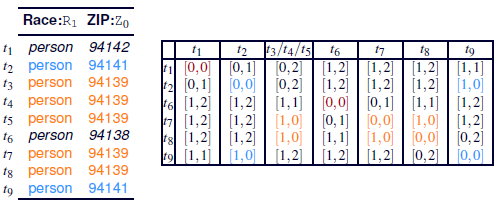
\includegraphics[scale=0.6]{img/dvmatrix2.png}
\end{center}
Soddisfa 2-anonymity sopprimendo t2 e t6\\\\
Ora supponiamo k=2 e MaxSup=2\\
Calcoliamo la prima soluzione ad altezza 1, quindi \(GT_{[1,0]}\) e \textbf{\(GT_{[0,1]}\)}
\begin{center}
    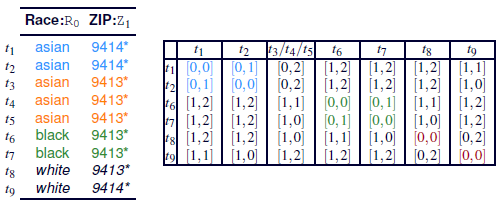
\includegraphics[scale=0.6]{img/dvmatrix3.png}
\end{center}
Soddisfa 2-anonymity sopprimendo t8 e t9\\\\

\subsubsection{k-Optimize algorithm}
Ordiniamo gli attributi nei QI (quasi identificatori) e i valori nel loro dominio. Successivamente associamo un valore intero ad ogni elemento del dominio, seguendo l'ordine crescente:
\begin{center}
    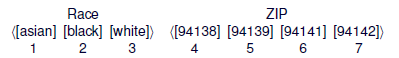
\includegraphics[scale=0.6]{img/koptim.png}
\end{center}
Una generalizzazione è l'unione di ogni valore degli indici.\\
L'ordinamento di tali valori ha impatto sul risultato della generalizzazione.\\
Quindi questo algoritmo produce dei cluster mettendo insieme valori che sono adiacenti. Quando l’algoritmo fa la generalizzazione andrà a mettere insieme i valori adiacenti. Rappresentazione come un insieme: se scrivo (4,6) significa l’insieme (4,5), cioè fino al 6 escluso, e l’insieme dal 6 in avanti (nel nostro esempio 6,7). Poi si mette tutto in un albero:
\begin{center}
    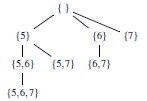
\includegraphics[scale=0.6]{img/koptimtree.png}
\end{center}
Possiamo notare come, passando dal nodo padre al nodo figlio vengono messi insieme gruppi che erano separati.\\
Ogni nodo ha un costo che rappresenta il numero di generalizzazioni e soppressioni dell'anonimizzazione rappresentata dal nodo stesso. Ogni tupla ha un costo associato che riflette la perdita di informazioni associata con la sua generalizzazione o soppressione.\\
Come facciamo a trovare la soluzione?\\
k-Optimize visita l'albero utilizzando il metodo depth first, cercando l'anonimizzazione col costo minore. Siccome il numero di nodi in un albero è \(2^{|I|}\) il costo della visita non è molto pratico: adottiamo quindi la tecnica di pruning dell'albero, ossia se il nodo n non va bene, neanche tutti i suoi figli andranno bene.\\
Questa determinazione può essere fatta calcolando un margine inferiore sul costo dei nodi nel sottoalbero che ha radice in n. Se il limite inferiore è maggiore del costo migliore trovato fino ad ora, scarto il nodo n e i suoi discendenti.\\\\
Il problema di questa soluzione è il concetto di adiacenza che non è detto che sia semanticamente rilevante.

\subsubsection{Incognito algorithm}
Incognito sfrutta questa proprietà: per avere le coppie uguali a due-a-due, anche i singoli valori devono comparire a due-a-due. Esempio: se voglio due occorrenze di Race e ZIP, ci devono essere due valori di R e due valori di Z. Questa è una condizione necessaria ma non sufficiente.\\
Incognito funziona a iterazioni:
\begin{itemize}
    \item \textbf{Iterazione 1:} controllo che k-anonymity sia rispettata per ogni attributo nei QI, scartando le generalizzazioni che non soddisfano k-anonymity
    \item \textbf{Iterazione 2:} combina le rimanenti generalizzazioni in coppia e controlla k-anonymity per ogni coppia ottenuta.
    \item ...
    \item \textbf{Iterazione i:} combino le generalizzazioni che soddisfano k-anonymity all'iterazione i-1 e controllo che sia rispettata k-anonymity per ogni i-upla ottenuta
    \item  \textbf{Iterazione \(|QI|\):} ritorna il risultato finale
\end{itemize}
Incognito usa un approccio bottom up per la visita di DGHS.
\begin{center}
    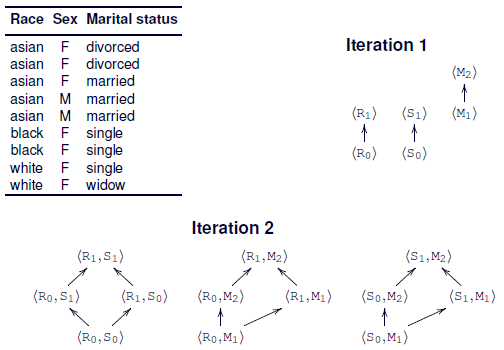
\includegraphics[scale=0.6]{img/inco1.png}
\end{center}
\begin{center}
    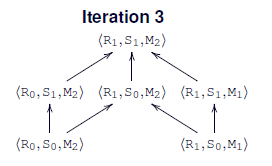
\includegraphics[scale=0.6]{img/inco2.png}
\end{center}
Incognito taglia lo spazio di soluzioni producendo una gerarchia di soluzioni semplificata, ma poi devo andare a cercare il minimo nella gerarchia (ad esempio con la binary search).

\subsubsection{Heuristic algorithm}
Gli algoritmi esatti hanno complessità esponenziale in proporzione a QI. Gli algoritmi euristici proposti sono:
\begin{itemize}
    \item basati su algoritmi genetici che risolvono il problema di k-anonymity usando un metodo di ricerca stocastico incompleto
    \item basati su simulated annealing per trovare soluzioni minime locali, ma richiedono un alto tempo di computazione e non garantiscono la qualità della soluzione
    \item algoritmi euristici top-down per ottenere una tabella k-anonima. Partono dalla soluzione più generale e ad ogni passo tendono a specificare alcuni valori fino a quando non viene violata k-anonymity
\end{itemize}
Con gli algoritmi euristici non posso specificare margini o bontà della soluzione che andrò a trovare, ma possiamo utilizzare i risultati per calcolare la qualità della soluzione trovata.

\subsection{Algoritmi per CS e CG}
Parliamo di algoritmi che operano a livello di cella effettuando soppressioni e generalizzazioni. Ovviamente questo è più oneroso.
\subsubsection{Mondrian multidimensional algorithm}
Ogni attributo che è un quasi identificatore QI raprresenta una dimensione.\\
Ogni tupla in PT rappresenta un punto nello spazio definito da QI.\\
Le tuple con lo stesso valore di QI sono rappresentate dando un valore multiplo al punto nello spazio.\\
Lo spazio multidimensionale è partizionato dividendo le dimensioni tali che ogni area contenga almeno k occorrenze per valore di punti.\\
Tutti i punti in una regione sono generalizzati con un unico valore.\\
Le tuple corrispondenti sono sostituite con quelle generalizzate.\\
L'algoritmo di Modrian è flessibile e può operare:
\begin{itemize}
    \item su diversi attributi
    \begin{itemize}
        \item singola dimensione
        \item dimensione multipla
    \end{itemize}
    
    \item con diverse strategie di generalizzazione:
    \begin{itemize}
        \item generalizzazioni globali
        \item generalizzazioni locali
    \end{itemize}
    
    \item con diverse strategie di partizionamento
    \begin{itemize}
        \item partizionamento stretto (non overlapping)
        \item partizionamento rilassato (potentially overlapping)
    \end{itemize}
    
    \item usando differenti metriche per determinare come dividere ogni dimensione
\end{itemize}
\begin{center}
    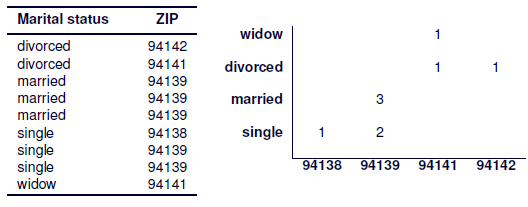
\includegraphics[scale=0.6]{img/modrian1.png}
\end{center}
Come possiamo notare dalla PT i valori vengono ordinati e viene fatto un grafico (numero di assi corrispondente al numero delle colonne) che rappresenta quanti punti ci sono in un determinato incrocio.\\
Come troviamo la soluzione supponendo di voler soddisfare 3-anonymity?\\
Devo tagliare lo spazio in modo tale da avere almeno k (nel nostro caso 3) punti per ogni sottospazio. 
\begin{center}
    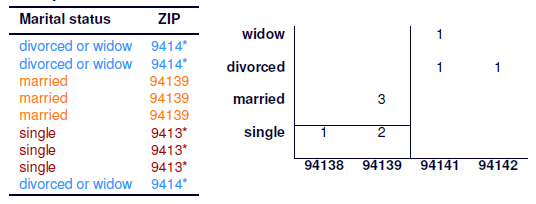
\includegraphics[scale=0.6]{img/modrian2.png}
\end{center}
Il vantaggio di questo algoritmo è che effettua il clustering ottimale senza dover specificare nulla in partenza. Uno svantaggio invece è quello che richiede un ordine totale sul dominio degli attributi e non è sempre possibile farlo.

\subsubsection{Approximation algorithm}
Non producono la soluzione ottimale ma quella che si avvicina di più a quella che desidero io (ad esempio 1,5-approximation per 2-anonymity)
\begin{itemize}
    \item algoritmi di approssimazione per CS
    \begin{itemize}
        \item \(O(klog(k))\)-approximation
        \item \(O(k)\)-approximation
    \end{itemize}
    \item algoritmi di approssimazione per CG
    \begin{itemize}
        \item \(O(k)\)-approximation
    \end{itemize}
\end{itemize}

\subsubsection{k-anonymity revisited}
Il requisito fondamentale di k-anonymity: per ogni rilascio di una tabella ci deve essere una combinazione di QI che deve almeno matchare k rispondenti.\\
Quando la generalizzazione è effettuata a livello di attributo questo è uguale a richiedere almeno k occorrenze per ogni valore del QI. \\
Quando la generealizzazione è effettuata a livello di cella, l'esistenza di almeno k occorrenze è sufficiente ma non è necessaria. In questo caso è sufficiente un requisito meno stringente:
\begin{itemize}
    \item per ogni sequenza di valori pt in PT[QI] ci sono almeno k tuple in GT[QI] che contiene una sequenza di valori che generalizzano pt
    \item per ogni sequenza di valori t in GT[QI] ci sono almeno k tuple in PT[QI] che contengono una sequenza di valori per i quali t è una generalizzazione
\end{itemize}
\begin{center}
    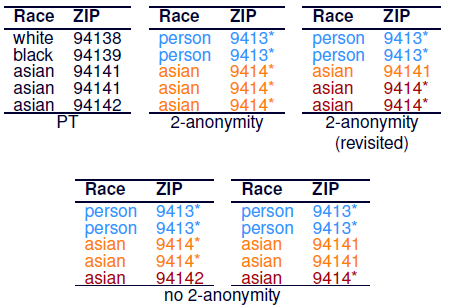
\includegraphics[scale=0.6]{img/kanonriv.png}
\end{center}
Con k-anonymity revisited dobbiamo per forza conoscere i dati di partenza per capire se sono protetti.
\clearpage
\subsection{Attribute disclosure}
k-anonymity è vulnerabile ad alcuni tipi di attacco. Prendiamo ad esempio questa tabella
\begin{center}
    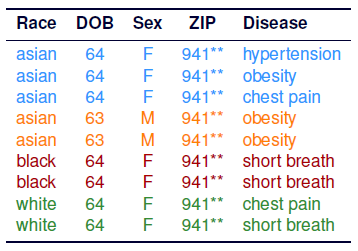
\includegraphics[scale=0.6]{img/kanonprob.png}
\end{center}
Gli arancio e i rossi sono esposti perchè i loro record sono uguali. Questo prende il nome di \textbf{problema dell'omogeneità}: se nascondo identità in un gruppo omogeneo dove tutti hanno la stessa informazione sensibile, allora non l'ho nascosta.\\
Un altro problema che posso incontrare è quello della \textbf{background/external knowledge}, che si basa su una conoscenza pregressa derivante anche da fonti esterne.\\
Ad esempio: un avversario sa che Hellen è una donna bianca e sa che i suoi dati sono in questa tabella. Sa anche che corre due ore al giorno quindi non può avere un problema di fiato corto (quindi da una incertezza di due passo a una incertezza di uno).

\subsubsection{l-diversity}
Un q-block (un insieme di tuple con gli stessi valori per i QI) in T è l-diverso se contiene almeno l "ben-rappresentati" valori diversi per gli attributi sensibili in T.
Con l-diversity un avversario deve eliminare almeno l-1 possibili valori per eseguire delle inferenze e capire che un rispondente rispecchia determinati valori.\\
Prendendo la tabella di prima: il gruppo blu è 3-diverso, quello verde è 2-diverso, quelli arancio e rosso sono 1-diversi.\\
Una tabella T si dice l-diversa se tutti i q-blocks sono l-diversi (l'attacco basato sull'omogeneità non è più possibile e l'attacco basato suy background knowledge diventa più difficile).\\
Anche l-diversity non risulta essere abbastanza, infatti è vulnerabile a diversi attacchi:
\begin{itemize}
    \item \textbf{skewness attack}: si verifica quando la distribuzione di q-block è differente (ha una distribuzione peculiare) rispetto alla distribuzione della popolazione
    \item \textbf{similarity attack}: si verifica quando i valori sono diversi ma semanticamente simili
\end{itemize}

\subsubsection{t-closeness}
Un q-block rispetta t-closeness se la distanza tra la distribuzione dei valori degli attributi sensibili nel q-block e nella popolazione considerata è meno di t.\\
T rispetta t-closeness se tutti i q-block rispettano t-closeness.\\
t-closeness è monotona con il rispoetto della gerarchia di generalizzazione considerata per lo scopo di k-anonymity.\\
t-closeness non è facile perché dipende dai nostri dati, può essere che per rispettare t-closeness i miei dati diventino inutilizzabili perché sono troppo generali.
\subsubsection{External knowledge}
La considerazione delle conoscenze pregresse che possono avere gli eventuali avversari è necessaria quando si ragiona sulla pubblicazione dei dati. Le conoscenze esterne possono essere utilizzate per effettuare:
\begin{itemize}
    \item \textbf{inferenze positive}: osservatore può scoprire che un rispondente ha un certo valore o ha uno di una manciata di valori. Questo caso è considerato il problema principale.
    \item \textbf{inferenze negative}: osservatore può scoprire che un rispondente non ha un certo valore. Generalmente non è considerato un problema ma ovviamente dipende dai dati. Solitamente viene usata come pezzo del puzzle per arrivare all’identificazione/inferenza.
\end{itemize}
Le informazioni che un attaccante può avere sono diverse e possono arrivare da altrettanti fonti diverse:
\begin{itemize}
    \item conoscenza rispetto alla persona (esempio: la persona corre due ore al giorno quindi non può avere fiato corto)
    \item conoscenza rispetto agli altri (esempio: se so che una persona non ha fiato corto, allora l’altra è esposta.)
    \item conoscenza rispetto agli altri correlati (esempio: DNA simile tra due persone)
\end{itemize}
Vediamo un esempio:
\begin{center}
    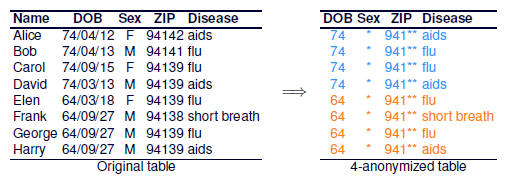
\includegraphics[scale=0.6]{img/exknow.png}
\end{center}
La tabella rilasciata è 4-anonima, ma l'avversario sa che Harry che è nato nel 64 e vive nell'area 94139 è nella tabella. Quindi Harry appartiene al gruppo arancio. Da un altro dataset l'avversario sa che George (nato nel 64, vive nell'area 941**) è nella tabella e ha l'influenza. Sempre da sue conoscenze personali l'avversario sa che Harry non ha il fiato corto, quindi l'attaccante può affermare con una confidenza del 50\% che Harry ha l'aids.

\subsubsection{Multiple releases}
I dati possono essere soggetti a variazioni frequenti e devono essere pubblicati di costante. Questi rilasci multipli possono causare dei leak delle informazioni siccome un utente malizioso potrebbe correlare questi dataset rilasciati. 
\begin{center}
    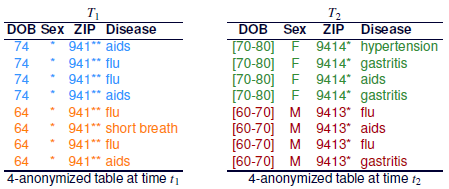
\includegraphics[scale=0.6]{img/multrel.png}
\end{center}
Come nel caso precedente, anche qui posso effettuare delle inferenze a partire anche da conoscenze pregresse e ritrovare la malattia di uno specifico paziente.\\
Come posso proteggermi da questo attacco?

\subsubsection{m-invariance}
Una sequenza di tabelle di microdati soddisfa m-invariance sse:
\begin{itemize}
    \item ogni classe di equivalenza include almeno m tuple
    \item nessun dato sensibile appare più di una volta in ogni classe di equivalenza
    \item per ogni tupla t, le classi di equivalenza di questa tupla t sono caratterizzate dallo stesso set di dati sensibili
\end{itemize}
La correlazione di tuple nella sequenza di tabelle non permette a un attaccante di associare meno di m differenti dati sensibili per ogni rispondente

\subsection{Riassunto delle tecniche viste e altri scenari}
\begin{itemize}
    \item k-anonymity: difendiamo l'identità dei rispondenti confondendoli in gruppi di almeno k elementi
    \item l-diversity: i gruppi devono avere informazione sensibile diversa altrimenti siamo soggetti ad attacchi di omogeneità
    \item t-closeness: i gruppi devono avere informazioni sensibili diverse (semanticamente) e con distribuzione il più possibile simile a quella della popolazione reale
\end{itemize}
Questi algoritmi sono basati su assunzioni che li rendono non sempre applicabili in scenari specifici:
\begin{itemize}
    \item più tuple che si riferiscono ad uno stesso individuo (ad esempio quando vado all'ospedale e faccio più esami): tecniche \(k^m -anonimity\)
    \item rilascio di tabelle multiple caratterizzate da dipendenze: tecniche multiR k-anonymity
    \item quasi identificatori multipli: tecniche butterfly
    \item non ho quasi identificatori predefiniti, infatti definire questi identificatori non è facile: tecniche \(k^m-anonymity\)
    \item rilascio di data stream: tecniche k-anonymity data stream
\end{itemize}
\subsection{Applicazioni k-anonymity}
k-anonymity può essere applicata ad altri contesti oltre che al rilascio di tabelle di microdati.
\subsubsection{Social Network}
I social network sono soggetti al neighborhood attack dove, data la versione de identificata  G' di un grafo G, si riesce a ridurre l'incertezza e a volte reidentificare chi sta dietro i singoli nodi.
\begin{center}
    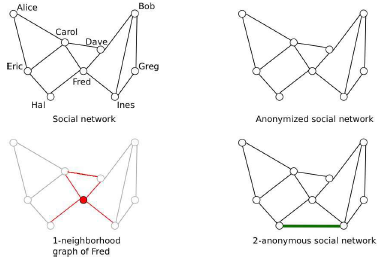
\includegraphics[scale=0.6]{img/anonsoc.png}
\end{center}
L'idea per proteggersi da questo attacco è quella di adattare k-anonymity:
\begin{itemize}
    \item un vertice u è k-anonimo se esistono almeno k-1 altri vertici \(v_1,...,v_\) tali che i sottografi tra i vicini di u e i vicini di \(v_1,...,v_\) siano isomorfi
    \item G' è k-anonimo se ogni vertice in G' è k-anonimo
    \item se G' è k-anonimo, ogni vertice in G non può essere reidentificato con una confidenza più grande di 1/k
\end{itemize}
\subsubsection{Data mining}
Privacy riguardo al data mining dipende dalla definizione di privacy a partire da quelle che sono le informazioni sensibili nei dati originali. k-anonymity in data mining ha l'obiettivo di garantire che il risultato del mining non violi k-anonymity.\\
Possono essere principalmente due i tipi di attacco nel mining:
\begin{itemize}
    \item regole di associazione: faccio mining sui dati per scoprire delle correlazioni nei dati
    \item regole di classificazione: stabilisco delle regole di classificazione che mi servono per classificare i nuovi dati.
\end{itemize}
Per proteggere la privacy dei rispondenti posso adottare due tecniche:
\begin{itemize}
    \item Anonymize and Mine: anonimizzo e poi rilascio la tabella dove chiunque può fare mining
    \begin{center}
    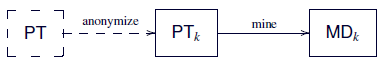
\includegraphics[scale=0.6]{img/a&m.png}
\end{center}
    \item Mine and Anonymize: faccio mining e poi anonimizzo
    \begin{center}
    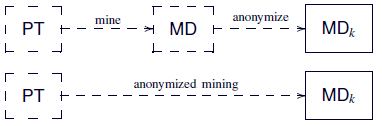
\includegraphics[scale=0.6]{img/m&a.png}
\end{center}
\end{itemize}
\subsubsection{Servizi di localizzazione}
Posso utilizzare anche la posizione come dato per carpire informazioni sensibili e in questo caso k-anonymity entra in gioco in modi diversi:
\begin{itemize}
    \item se la localizzazione espone l'identità: allargo l'area fino ad avere almeno k-1 individui
    \item se il luogo è sensibile: offusco l'area per diminuire la precisione
    \item se la traiettoria della persona è sensibile: creo incertezza nel percorso, offuscando un pezzo
\end{itemize}

\subsubsection{Tipi di privacy}
\textbf{Sintattica}: la definizione di privacy deve soddisfare un certo grado espresso con un numero, ciascun rilascio di dati non può essere riferito a un certo numero ristretto di individui che mi renda comfortable rispetto alla privacy che ho\\
\textbf{Semantica}: le definizioni di privacy sono basate sulla soddisfazione di un requisito semantico di privacy scelto in base al meccanimo del rilascio dei dati, quelli che analizzano i dati vedono un risultato che è indipendente dalla presenza o meno di qualcuno.\\
\textbf{Differenziale}: ha lo scopo di prevenire la capacità di rilevare la presenza o l'assenza di un individuo in un determinato dataset da parte degli avversari. La probabilità di distribuzione dei risultati (cioè il risultato dell’analisi) è essenzialmente la stessa indipendentemente dalla presenza di un individuo. Questa è possibile applicarla essenzialmente a due scenari: 
\begin{itemize}
    \item interattivo: vengono valutate a runtime le query
    \item non interattivo: vengono rilasciate tabelle di macrodati dove sono già stati fatti dei calcoli
\end{itemize}
E'imposta tendenzialmente aggiungendo rumore casuale ai dati, ma così facendo la veridicità dei dati non è preservata.

\subsubsection{k-anonimity vs privacy differenziale}
Ognuna delle due ha vantaggi e svantaggi:
\begin{center}
    \begin{tabular}{ |c|c|c| } 
        \hline
        & Vantaggi & Svantaggi  \\
        \hline
        k-anonimity & protegge l'info sensibile & non fornisce protezione completa \\ 
        \hline
        differential privacy & garantisce più protezione & implementazione più difficile \\ 
        \hline
    \end{tabular}
\end{center}
\subsection{Altri problemi di Privacy}
\subsubsection{Distribuzione di valori sensibili}
Le singole tuple non sono sensibili, ma l'unione di più tuple potrebbe generare un leak di informazioni sensibili (che nel mio dataset non erano rappresentati).\\
Esempio: dati medici dei militari; il dato medico del singolo militare non è sensibile. Ma se io guardo l’età posso inferire il tipo di locazione: se sono giovani è un campo di addestramento, se sono vecchi è un quartier generale. Il tipo di locazione è sensibile.
\begin{center}
    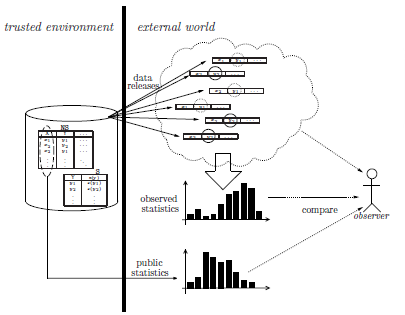
\includegraphics[scale=0.6]{img/sensvaldist.png}
\end{center}
In questo caso si genera un canale di inferenza tra età e posizione. Per contrastare questo canale dobbiamo capire qual è l'informazione sensibile e quando forzare il controllo di esposizione per limitare falsi positivi.
\subsubsection{Privacy e dati genomici}
I dati genomici sono una grande opportunità per la medicina ma a livello di privacy creano non pochi problemi perchè:
\begin{itemize}
    \item identificano il proprietario
    \item contengono informazioni su ereditarietà etnica, predisposizione a malattie ...
    \item espongono non solo il proprietario, ma anche i parenti e i discendenti
\end{itemize}
\subsubsection{Inferenza dal Data Mining}
Esempio reale: una catena di supermercati aveva capito che una ragazza fosse incinta in base agli acquisti. La profilazione ci dice molto di più di quello che c’è nei dati.\\
Inferenze dai social networks: non è solo quello che io dico, ma anche quello che dicono quelli vicini a me.